\documentclass[border=8pt]{standalone}
\usepackage{fontspec}\setmainfont{Times New Roman}
\usepackage{amsmath}\usepackage{tikz}
\usetikzlibrary{shapes.geometric, arrows.meta, positioning, calc}
\begin{document}
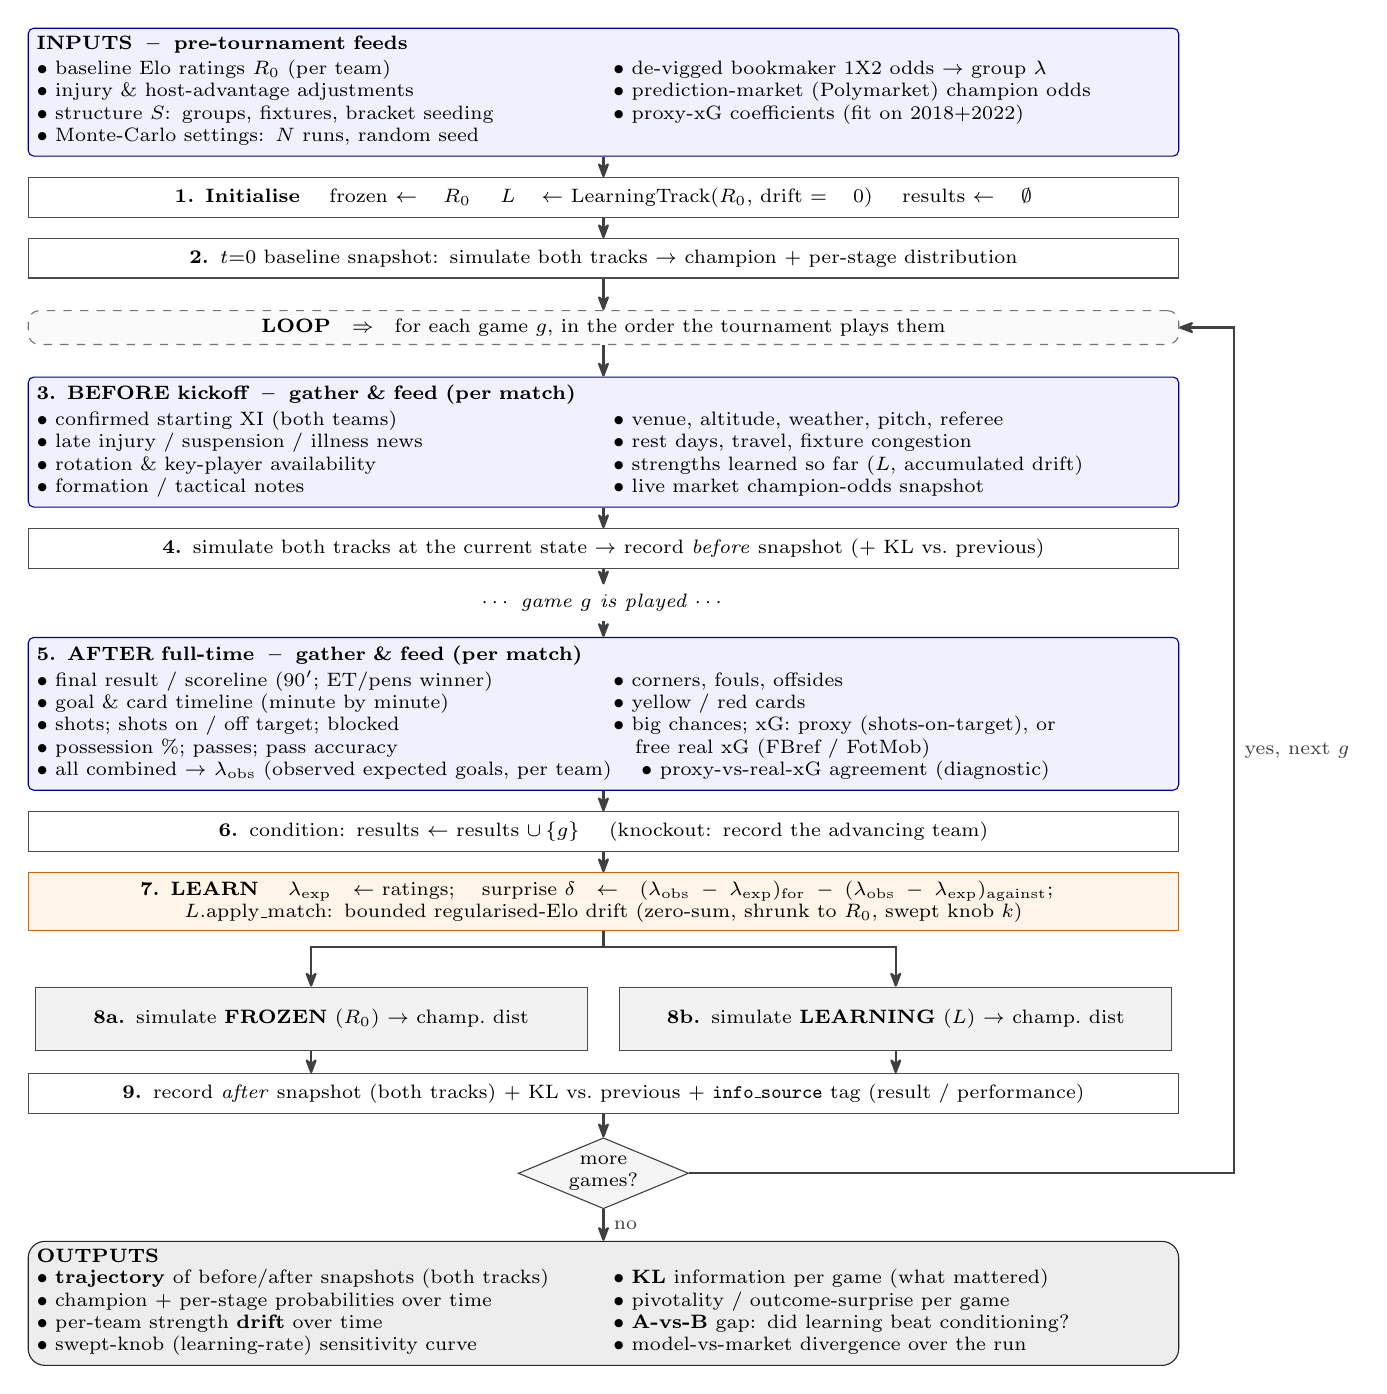
\begin{tikzpicture}[
  font=\scriptsize,
  >={Stealth[round]},
  io/.style={rectangle, rounded corners=2pt, draw=blue!55!black, fill=blue!6, align=left, text width=144mm, inner sep=3pt},
  pbox/.style={rectangle, draw=black!70, fill=white, align=center, text width=144mm, inner sep=3pt, minimum height=5mm},
  learn/.style={rectangle, draw=orange!80!black, fill=orange!9, align=center, text width=144mm, inner sep=3pt},
  sim/.style={rectangle, draw=black!70, fill=black!5, align=center, text width=68mm, inner sep=3pt, minimum height=8mm},
  dec/.style={diamond, draw=black!75, fill=black!4, aspect=2.4, align=center, inner sep=1pt},
  term/.style={rectangle, rounded corners=6pt, draw=black!85, fill=black!7, align=left, text width=144mm, inner sep=3pt},
  a/.style={->, thick, black!75},
  node distance=2.6mm,
]
\node[io] (inp) {\textbf{INPUTS \;\textendash\; pre-tournament feeds}\\[1pt]
\begin{tabular}{@{}p{69mm}p{69mm}@{}}
$\bullet$ baseline Elo ratings $R_0$ (per team) & $\bullet$ de-vigged bookmaker 1X2 odds $\to$ group $\lambda$\\
$\bullet$ injury \& host-advantage adjustments & $\bullet$ prediction-market (Polymarket) champion odds\\
$\bullet$ structure $S$: groups, fixtures, bracket seeding & $\bullet$ proxy-xG coefficients (fit on 2018+2022)\\
$\bullet$ Monte-Carlo settings: $N$ runs, random seed & \\
\end{tabular}};
\node[pbox, below=of inp] (init) {\textbf{1. Initialise} \quad frozen $\leftarrow R_0$ \quad $L \leftarrow$ LearningTrack($R_0$, drift $=0$) \quad results $\leftarrow \emptyset$};
\node[pbox, below=of init] (t0) {\textbf{2.} $t{=}0$ baseline snapshot: simulate both tracks $\rightarrow$ champion $+$ per-stage distribution};
\node[draw=black!55, dashed, fill=black!2, rounded corners, below=4mm of t0, text width=144mm, align=center, inner sep=3pt] (loophead) {\textbf{LOOP} \; $\Rightarrow$ \; for each game $g$, in the order the tournament plays them};
\node[io, below=4mm of loophead] (bef) {\textbf{3. BEFORE kickoff \;\textendash\; gather \& feed (per match)}\\[1pt]
\begin{tabular}{@{}p{69mm}p{69mm}@{}}
$\bullet$ confirmed starting XI (both teams) & $\bullet$ venue, altitude, weather, pitch, referee\\
$\bullet$ late injury / suspension / illness news & $\bullet$ rest days, travel, fixture congestion\\
$\bullet$ rotation \& key-player availability & $\bullet$ strengths learned so far ($L$, accumulated drift)\\
$\bullet$ formation / tactical notes & $\bullet$ live market champion-odds snapshot\\
\end{tabular}};
\node[pbox, below=of bef] (befsim) {\textbf{4.} simulate both tracks at the current state $\rightarrow$ record \emph{before} snapshot ($+$ KL vs.\ previous)};
\node[font=\scriptsize\itshape, below=2mm of befsim] (play) {$\cdots$ game $g$ is played $\cdots$};
\node[io, below=2mm of play] (aft) {\textbf{5. AFTER full-time \;\textendash\; gather \& feed (per match)}\\[1pt]
\begin{tabular}{@{}p{69mm}p{69mm}@{}}
$\bullet$ final result / scoreline (90$'$; ET/pens winner) & $\bullet$ corners, fouls, offsides\\
$\bullet$ goal \& card timeline (minute by minute) & $\bullet$ yellow / red cards\\
$\bullet$ shots; shots on / off target; blocked & $\bullet$ big chances; xG: proxy (shots-on-target), or\\
$\bullet$ possession \%; passes; pass accuracy & \quad free real xG (FBref / FotMob)\\
\multicolumn{2}{@{}l}{$\bullet$ all combined $\rightarrow$ $\lambda_{\text{obs}}$ (observed expected goals, per team) \quad $\bullet$ proxy-vs-real-xG agreement (diagnostic)}\\
\end{tabular}};
\node[pbox, below=of aft] (cond) {\textbf{6.} condition: results $\leftarrow$ results $\cup\,\{g\}$ \quad (knockout: record the advancing team)};
\node[learn, below=of cond] (learn) {\textbf{7. LEARN} \quad $\lambda_{\text{exp}} \leftarrow$ ratings; \;\; surprise $\delta \leftarrow (\lambda_{\text{obs}}-\lambda_{\text{exp}})_{\text{for}} - (\lambda_{\text{obs}}-\lambda_{\text{exp}})_{\text{against}}$; \;\; $L.\text{apply\_match}$: bounded regularised-Elo drift (zero-sum, shrunk to $R_0$, swept knob $k$)};
\node[sim, below left=7mm and 2mm of learn.south] (simf) {\textbf{8a.} simulate \textbf{FROZEN} ($R_0$) $\rightarrow$ champ.\ dist};
\node[sim, below right=7mm and 2mm of learn.south] (siml) {\textbf{8b.} simulate \textbf{LEARNING} ($L$) $\rightarrow$ champ.\ dist};
\node[pbox, below=7mm of learn, yshift=-11mm] (snap) {\textbf{9.} record \emph{after} snapshot (both tracks) $+$ KL vs.\ previous $+$ \texttt{info\_source} tag (result / performance)};
\node[dec, below=3mm of snap] (more) {more\\ games?};
\node[term, below=4mm of more] (out) {\textbf{OUTPUTS}\\[1pt]
\begin{tabular}{@{}p{69mm}p{69mm}@{}}
$\bullet$ \textbf{trajectory} of before/after snapshots (both tracks) & $\bullet$ \textbf{KL} information per game (what mattered)\\
$\bullet$ champion $+$ per-stage probabilities over time & $\bullet$ pivotality / outcome-surprise per game\\
$\bullet$ per-team strength \textbf{drift} over time & $\bullet$ \textbf{A-vs-B} gap: did learning beat conditioning?\\
$\bullet$ swept-knob (learning-rate) sensitivity curve & $\bullet$ model-vs-market divergence over the run\\
\end{tabular}};
% arrows
\draw[a] (inp)--(init);
\draw[a] (init)--(t0);
\draw[a] (t0)--(loophead);
\draw[a] (loophead)--(bef);
\draw[a] (bef)--(befsim);
\draw[a] (befsim)--(play);
\draw[a] (play)--(aft);
\draw[a] (aft)--(cond);
\draw[a] (cond)--(learn);
\draw[a] (learn.south)-- ++(0,-2mm) -| (simf.north);
\draw[a] (learn.south)-- ++(0,-2mm) -| (siml.north);
\draw[a] (simf.south) -- (simf.south|-snap.north);
\draw[a] (siml.south) -- (siml.south|-snap.north);
\draw[a] (snap)--(more);
\draw[a] (more)--(out) node[midway,right,font=\scriptsize]{no};
% loop back on the right
\draw[a] (more.east) -- ([xshift=7mm]bef.east|-more) -- ([xshift=7mm]bef.east|-loophead) node[midway,right,font=\scriptsize]{yes, next $g$} -- (loophead.east);
\end{tikzpicture}
\end{document}
